\subsubsection{Insertion}

When insert a data into the empty table (Figure \ref{fig:algorithm:string:insertion:empty_table}), every data will assign a unique \textit{id} for this data, this \textit{id} will use for the index to look for.

\begin{figure}[h]
\centering
%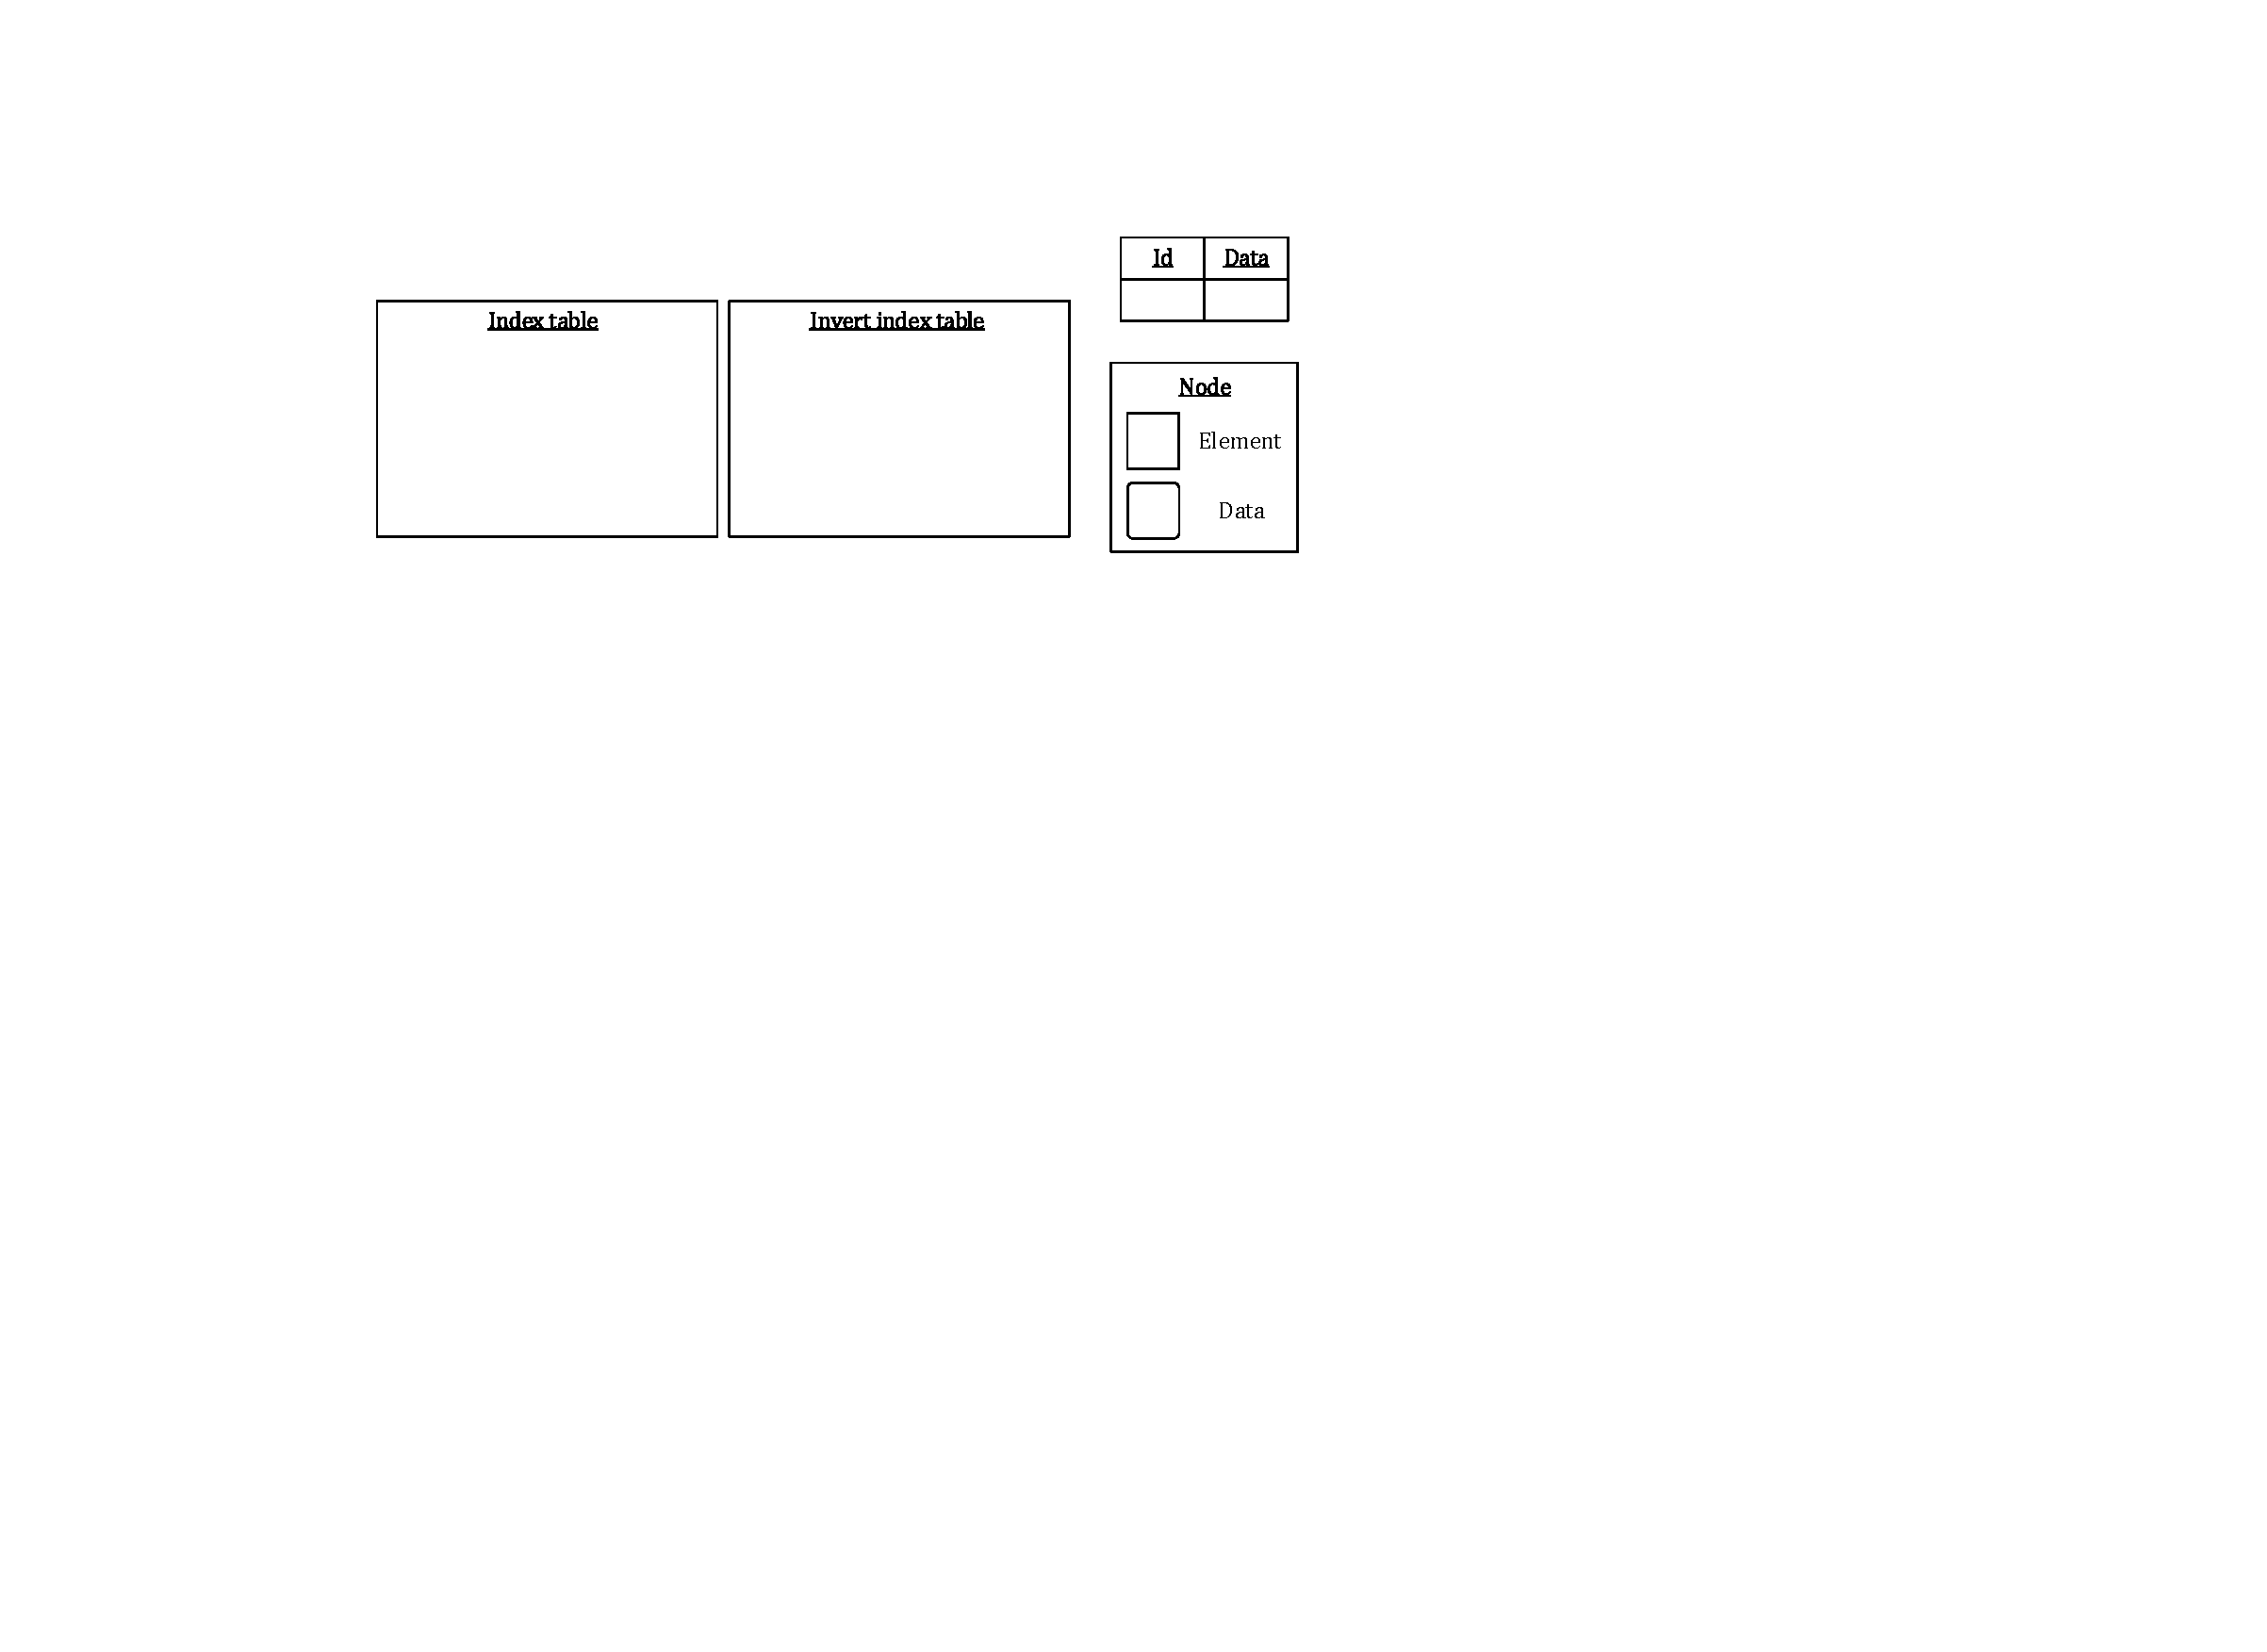
\includegraphics[scale=0.4]{./algorithm/string/pic/insertion/empty_table_v2.pdf}
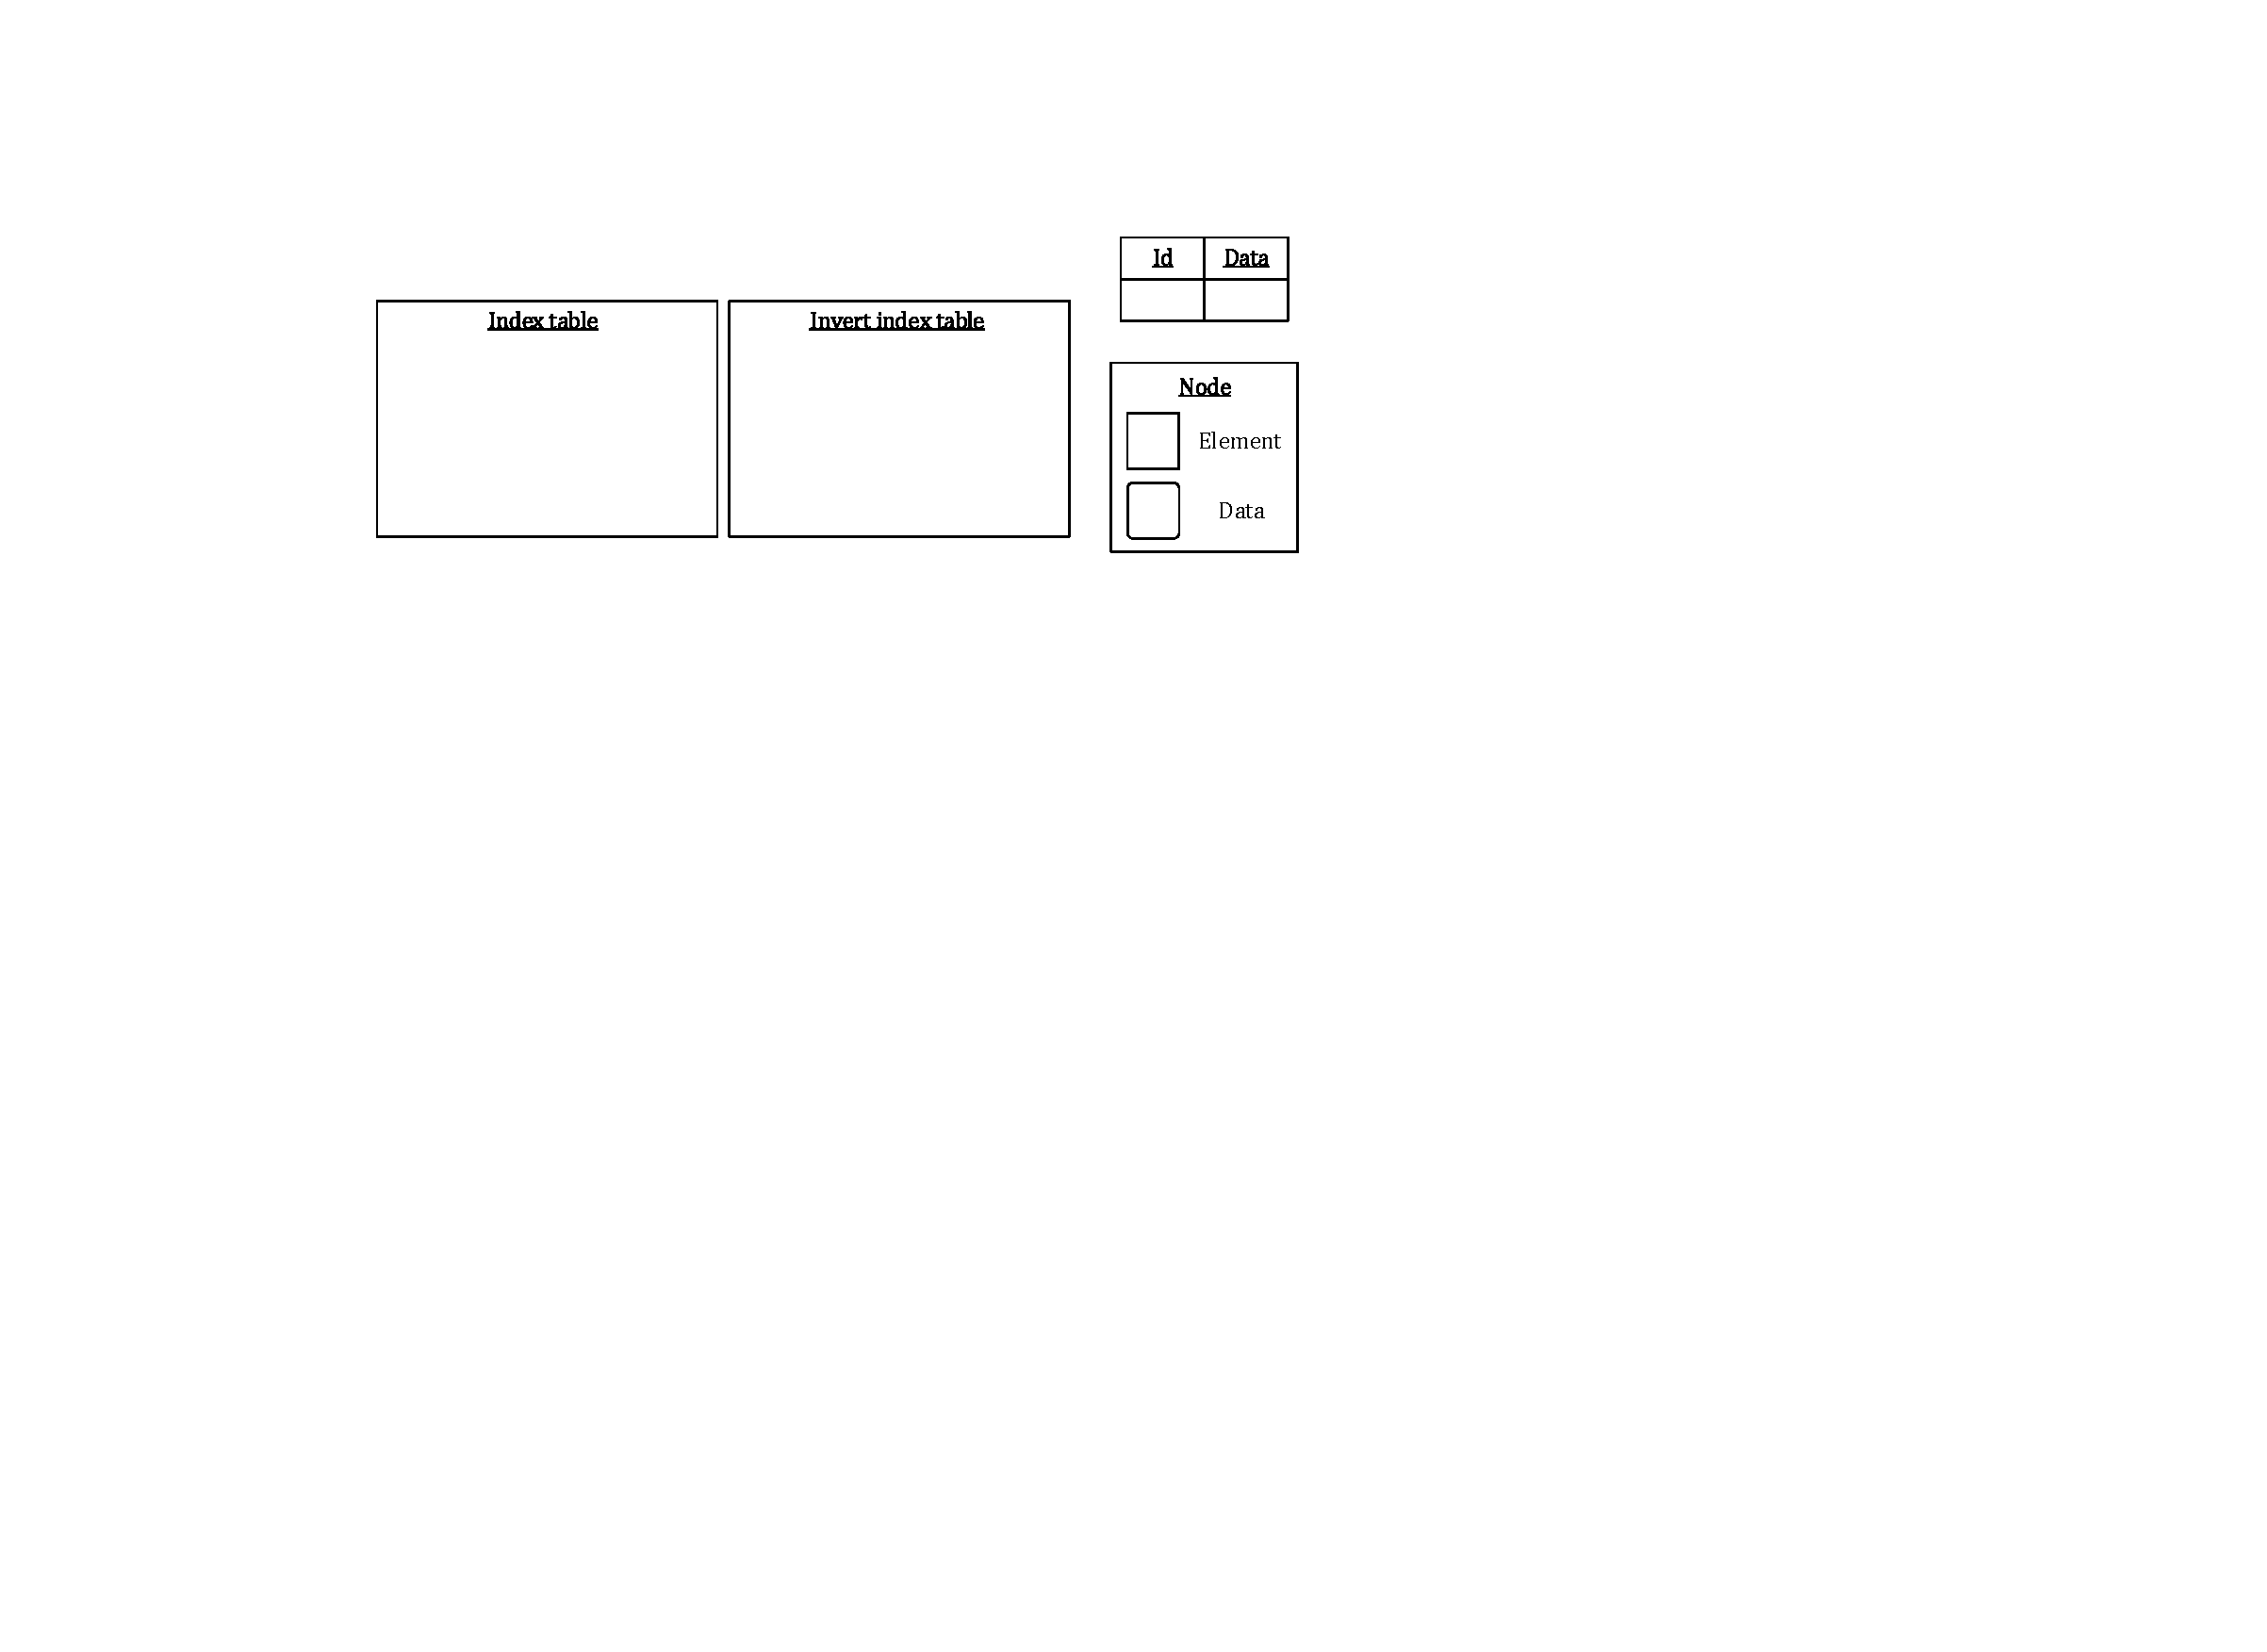
\includegraphics[width=0.5\textwidth]{./algorithm/string/pic/insertion/empty_table_v2.pdf}
\caption{A empty index table.}
\label{fig:algorithm:string:insertion:empty_table}
\end{figure}

So for example if inputting a data \textit{"book"}, first assign the \textit{id} as \textit{"\_d\_1\_"}, next step is separate the bytes using n-gram indexing with counting the repeat value to from the keys. So \textit{"book"} can count as \textit{b-\textgreater1}, \textit{o-\textgreater2} and \textit{k-\textgreater1} by counting the repeat value. And formed into \textit{"b"}, \textit{"bo"}, \textit{"boo"}, \textit{"book"}, \textit{"oo"}, \textit{"ook"} by n-gram but because using count the repeat byte that \textit{"bo"} is domained by \textit{"boo"}.\\

Every byte will have their own key such as \textit{'b'} and \textit{'o'} for record their repeat count, which is using in searching to know there have the keys like \textit{"'b':r1"} or \textit{"'o':r2"} which can use. The \textit{'r'} in key means the repeat times of that value. But the last byte wouldn't have that key in index table because of the key will exist in invert index table, also this happen in the opposite.\\

So the data will index as figure \ref{fig:algorithm:string:insertion:example_1}.

\begin{figure}[h]
\centering
%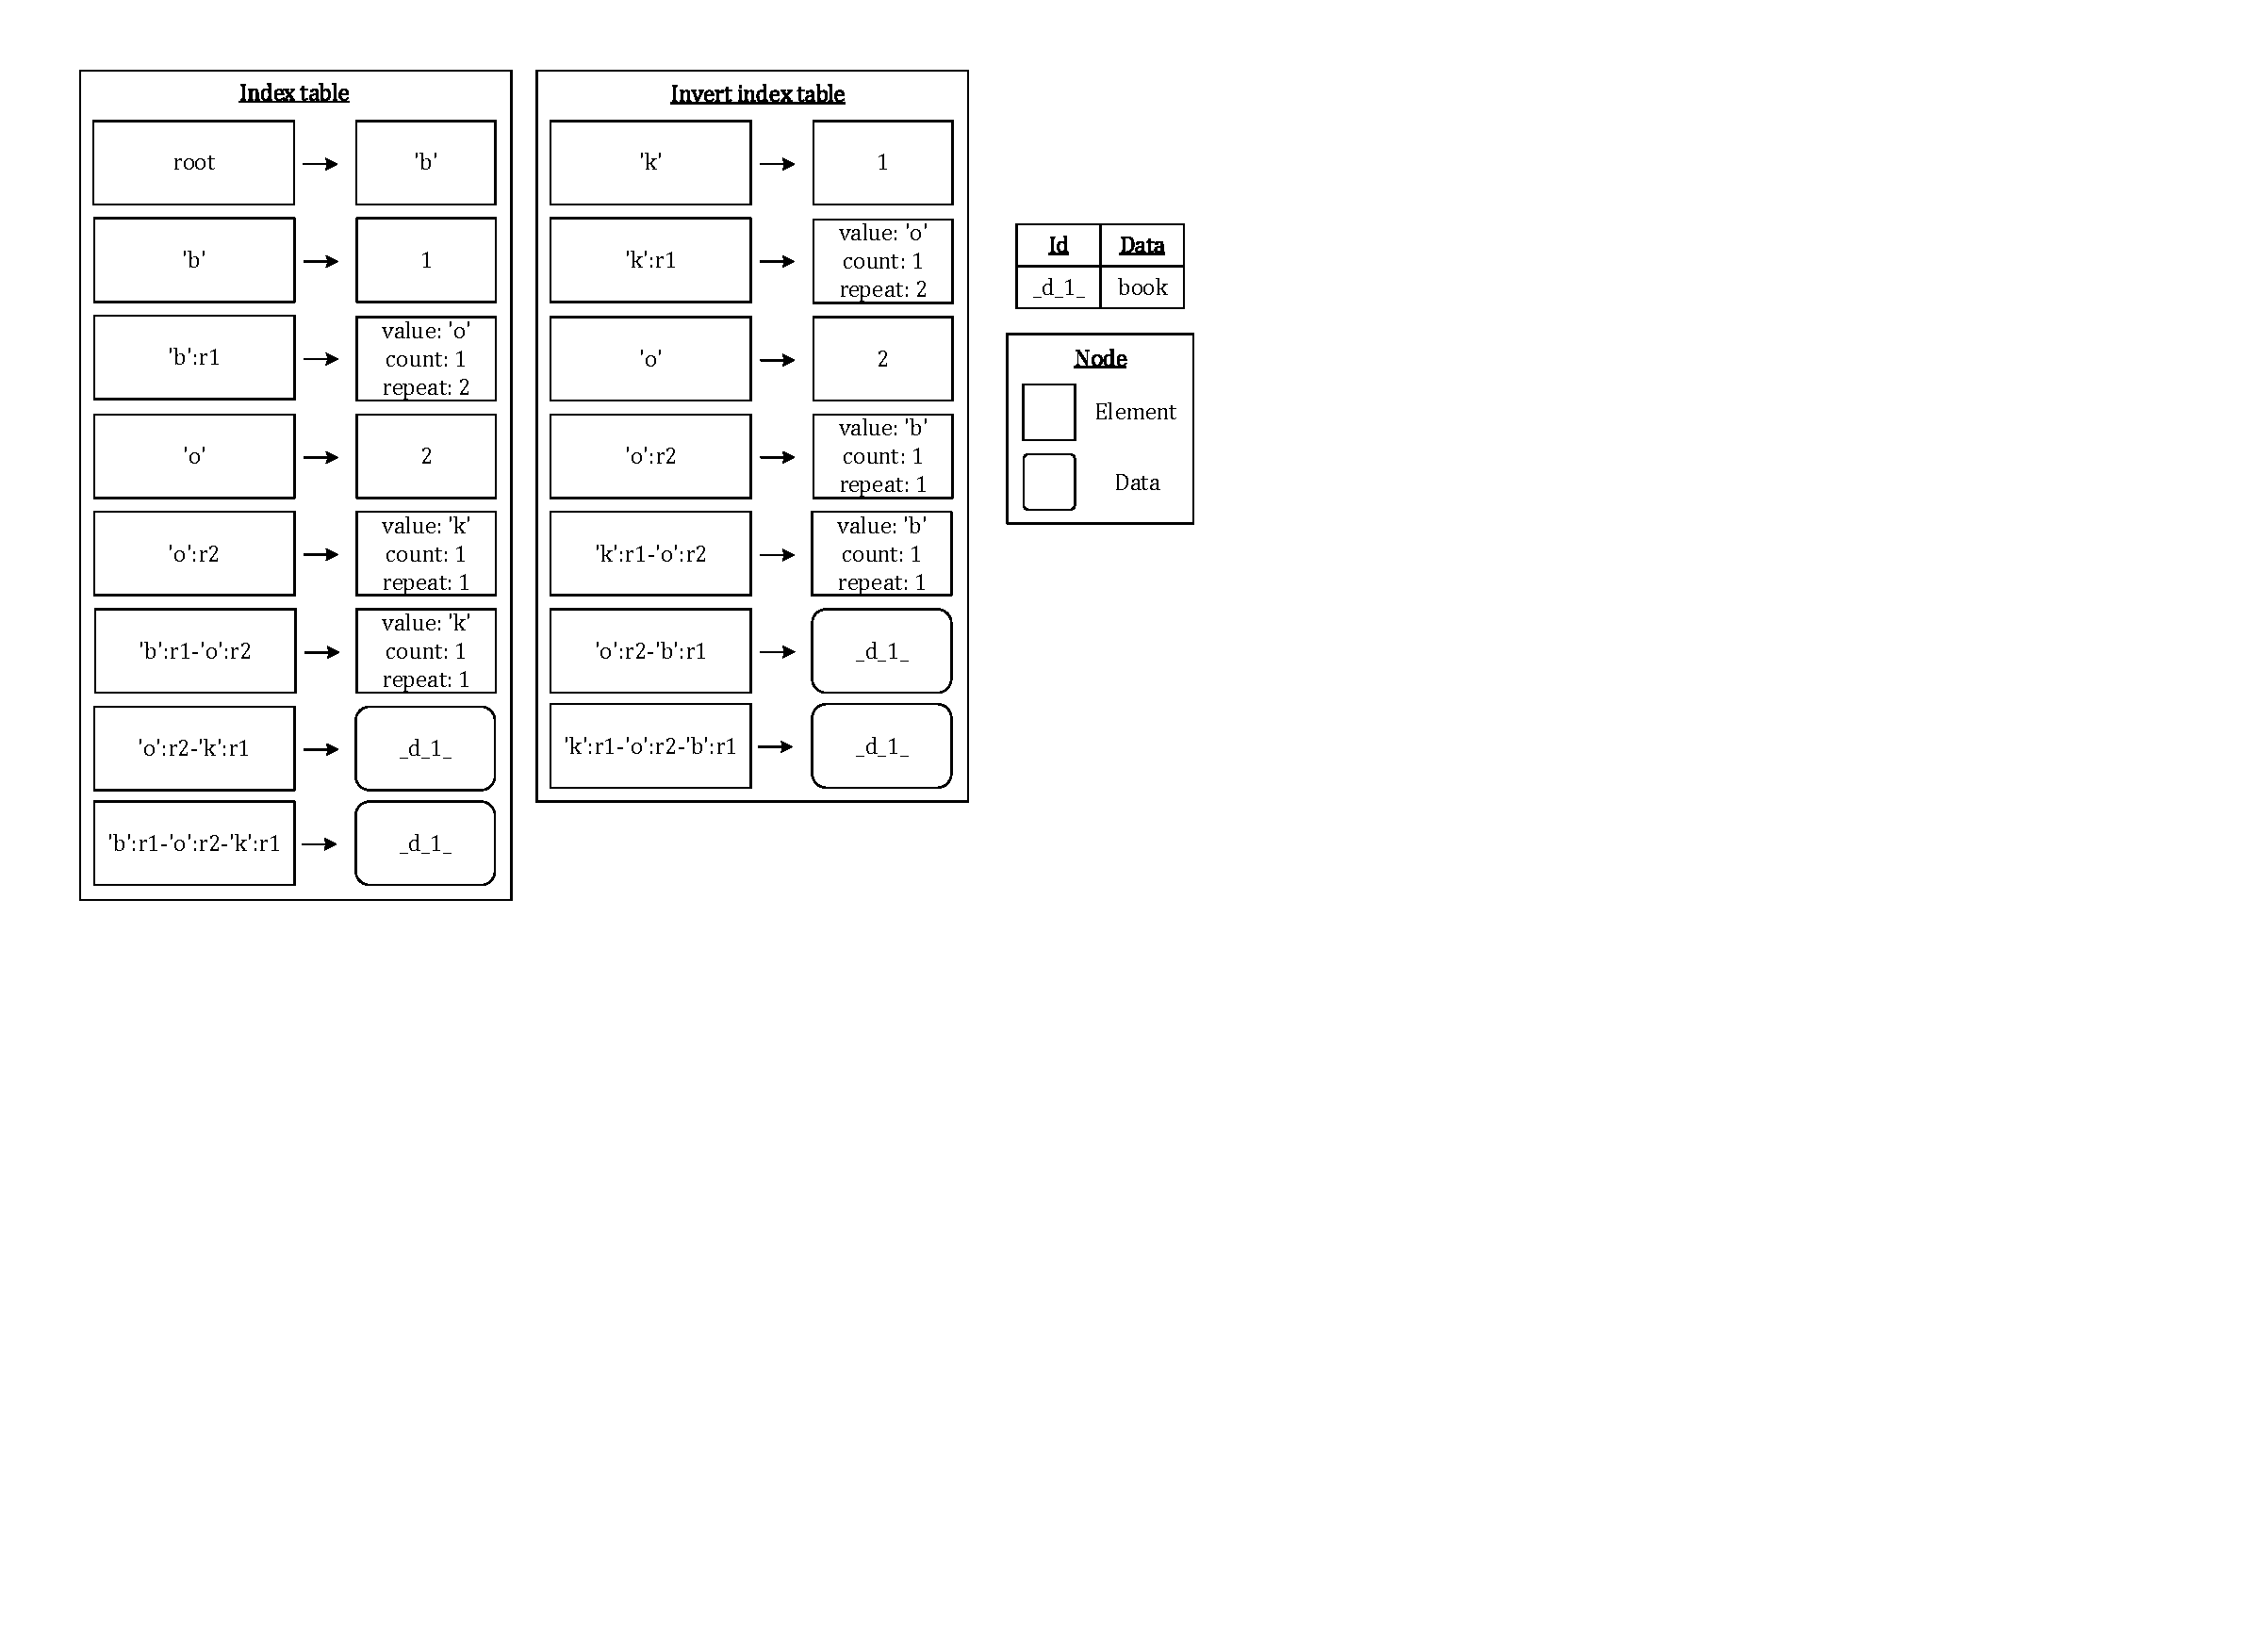
\includegraphics[scale=1.0]{./algorithm/string/pic/insertion/example_1_v5.pdf}
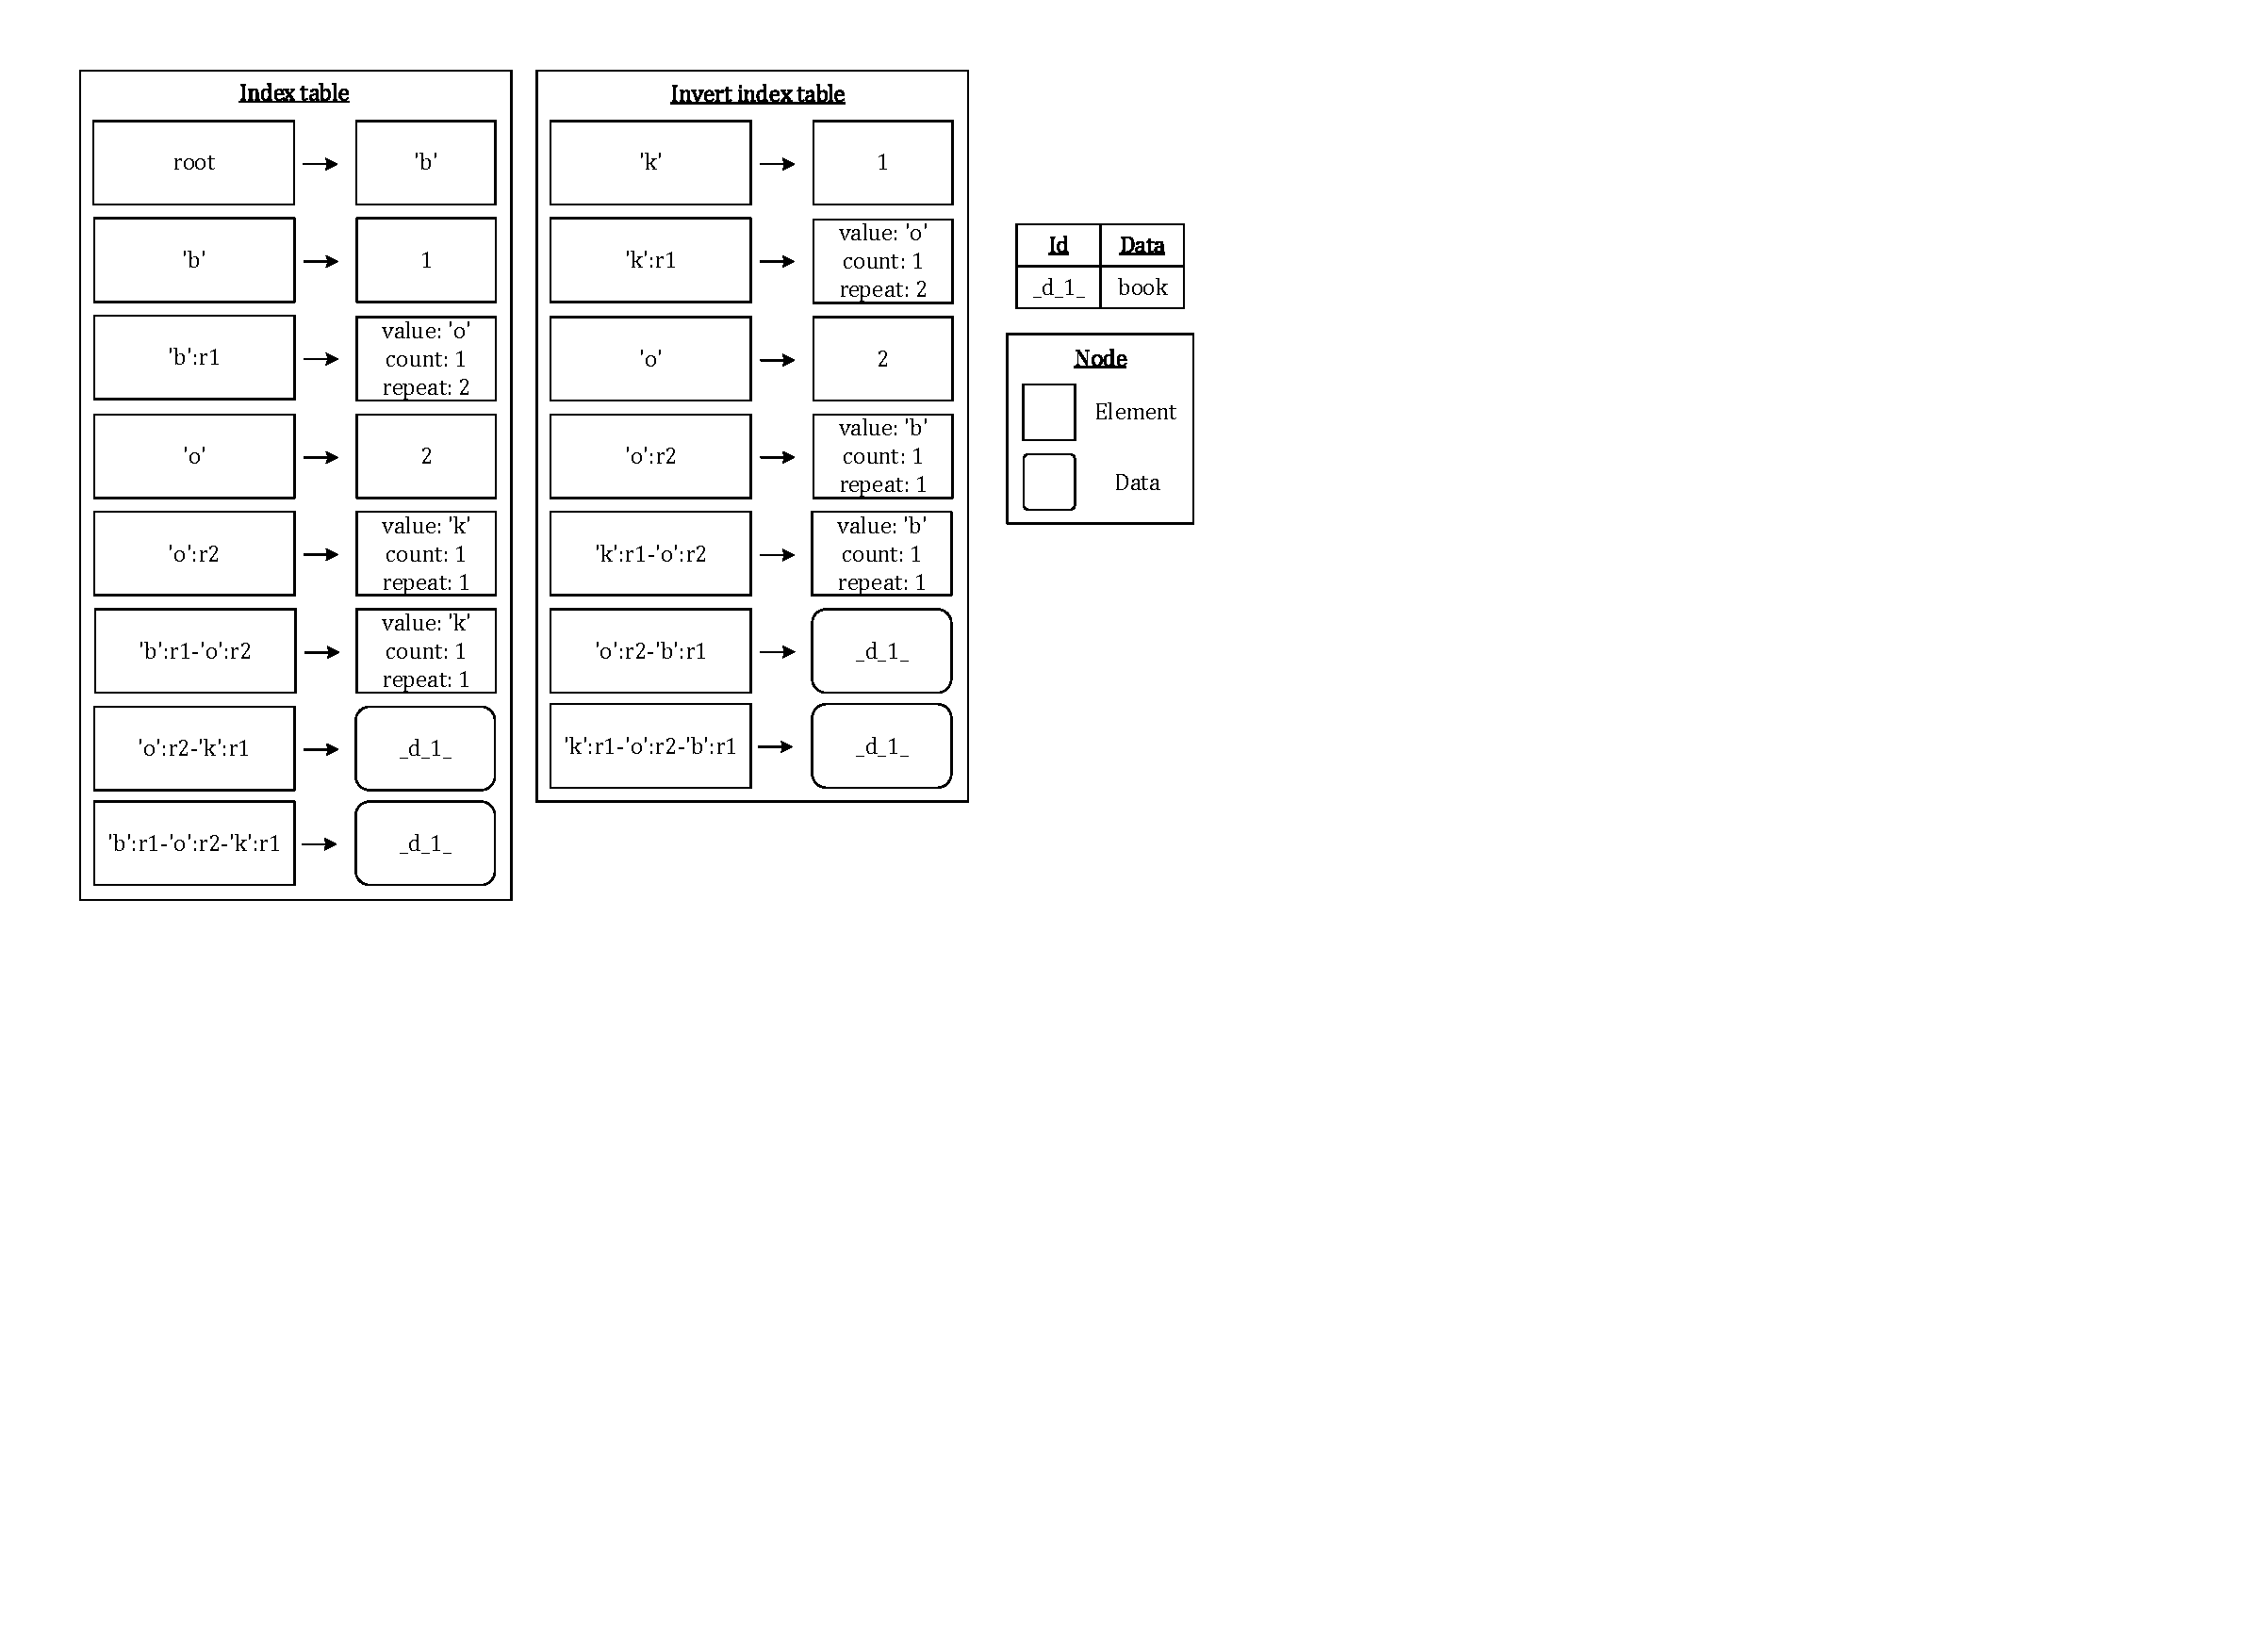
\includegraphics[width=0.7\textwidth]{./algorithm/string/pic/insertion/example_1_v5.pdf}
\caption{Insert data "book".}
\label{fig:algorithm:string:insertion:example_1}
\end{figure}

The time complexity of insertion should look like figure \ref{fig:algorithm:string:insertion:time_complexity}. The time complexity of insert a data should be $O(b)$, $b!$ is the number of for loop which is equal to the byte length of data, and $O(1)$ is means the key of the data like \textit{"'b':r1-'o':r2-'k':r1"} in the example.\\

\begin{figure}[h]
\centering
%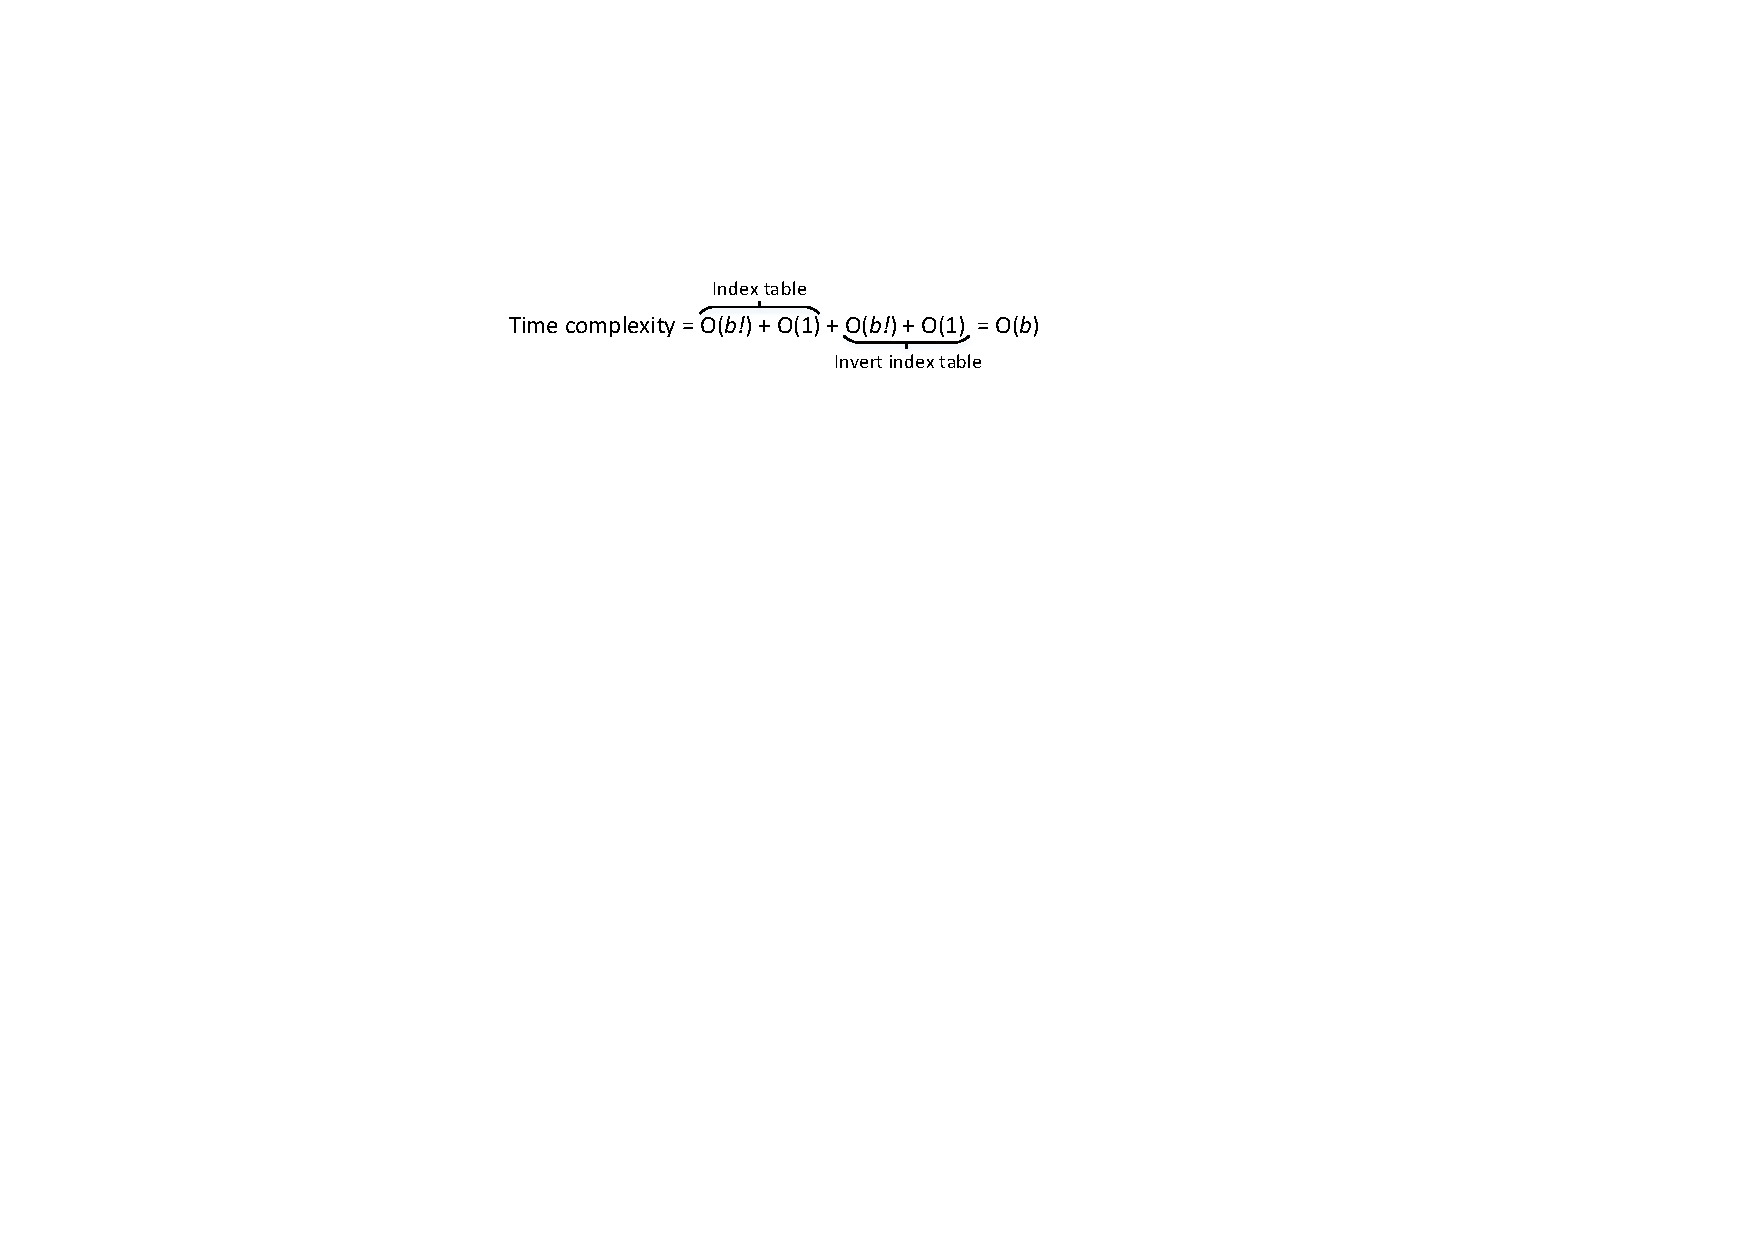
\includegraphics[scale=1.0]{./algorithm/string/pic/insertion/time_complexity_v5.pdf}
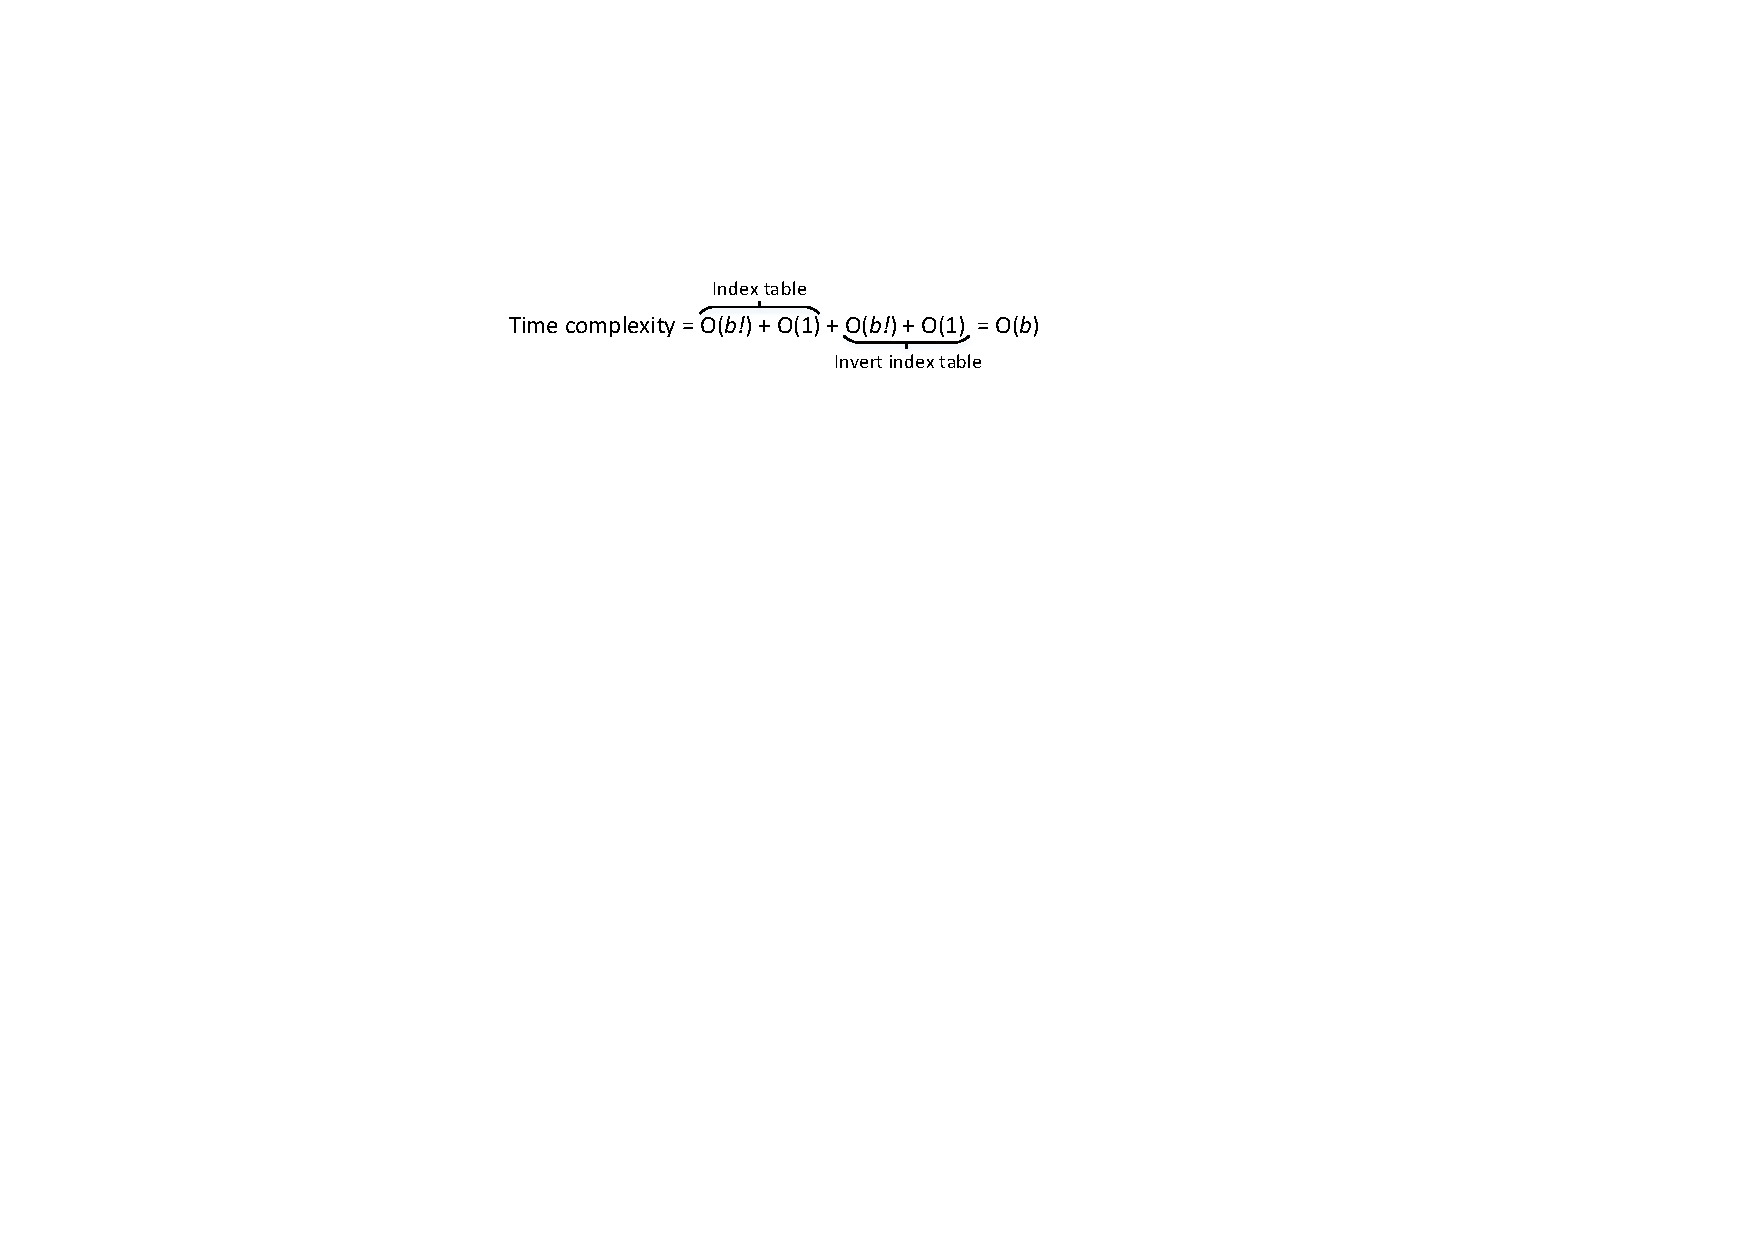
\includegraphics[width=0.6\textwidth]{./algorithm/string/pic/insertion/time_complexity_v5.pdf}
\caption{Time complexity of insertion.}
\label{fig:algorithm:string:insertion:time_complexity}
\end{figure}

Next if insert the data \textit{"box"}, the tables will look like figure \ref{fig:algorithm:string:insertion:example_2}. As the figure shows that \textit{"box"} and \textit{"book"} have a common key, so some of the node will deduplicated.

\begin{figure}[h]
\centering
%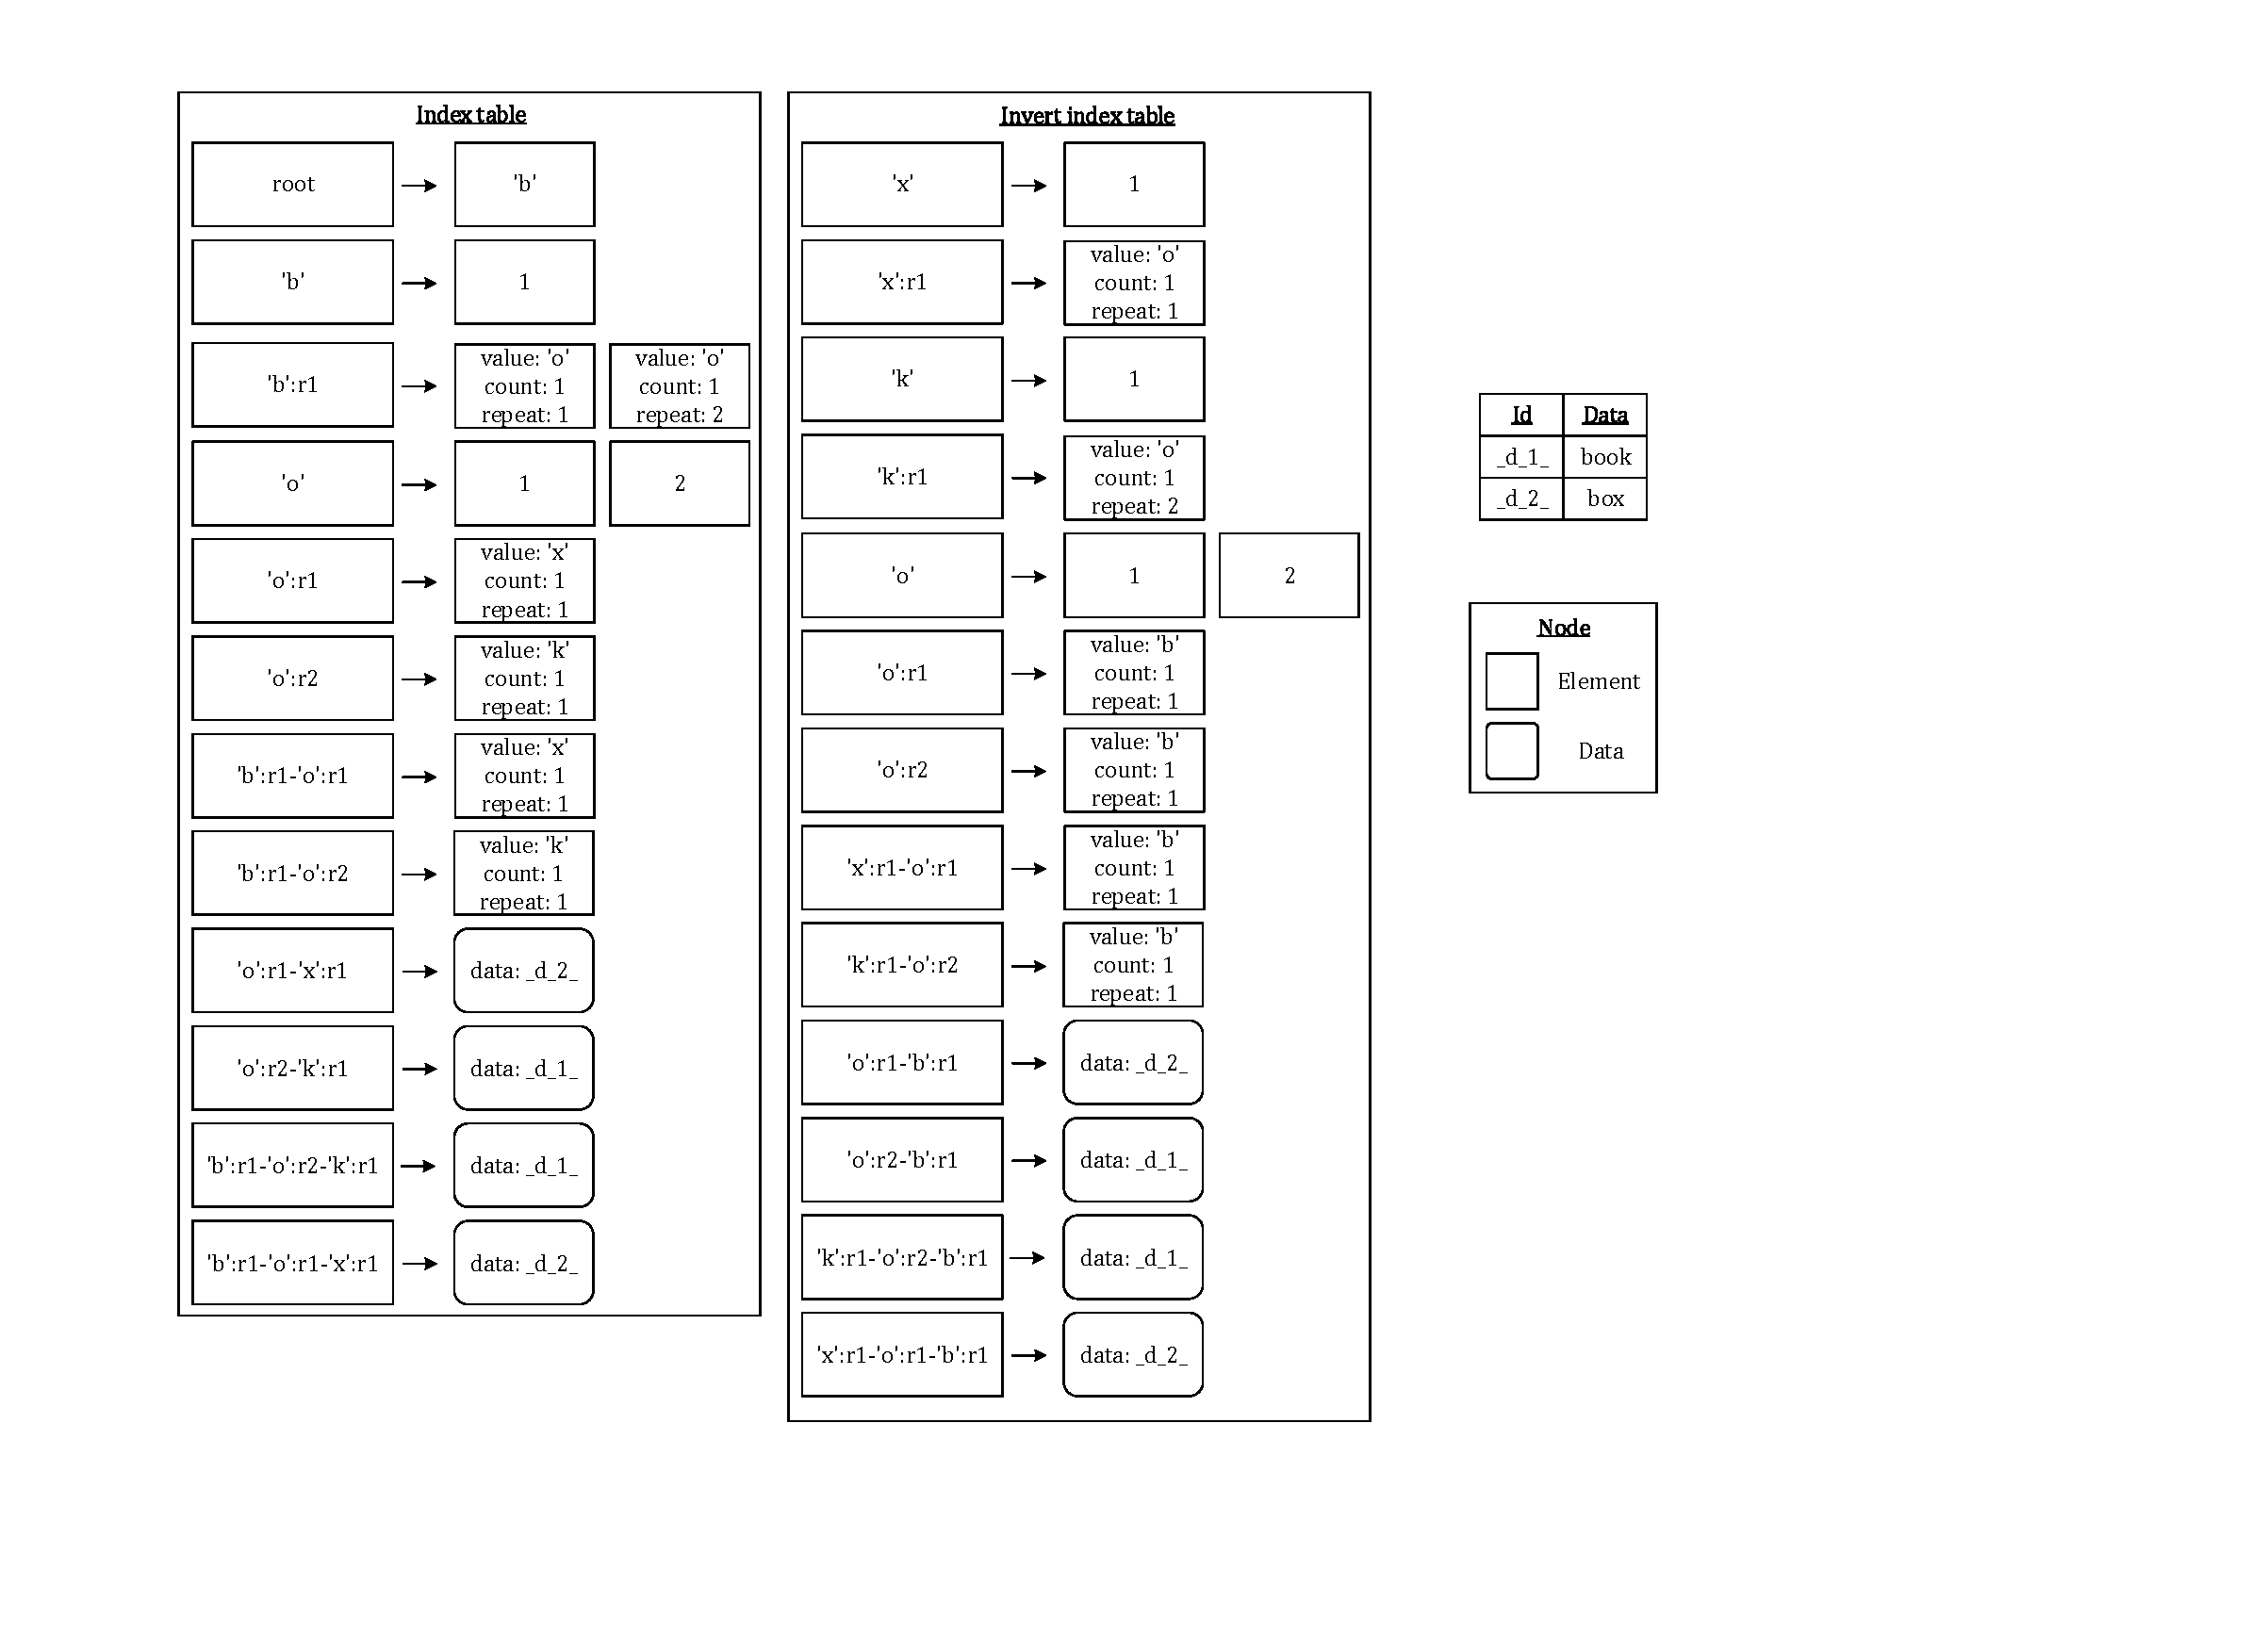
\includegraphics[scale=0.6]{./algorithm/string/pic/insertion/example_2_v5.pdf}
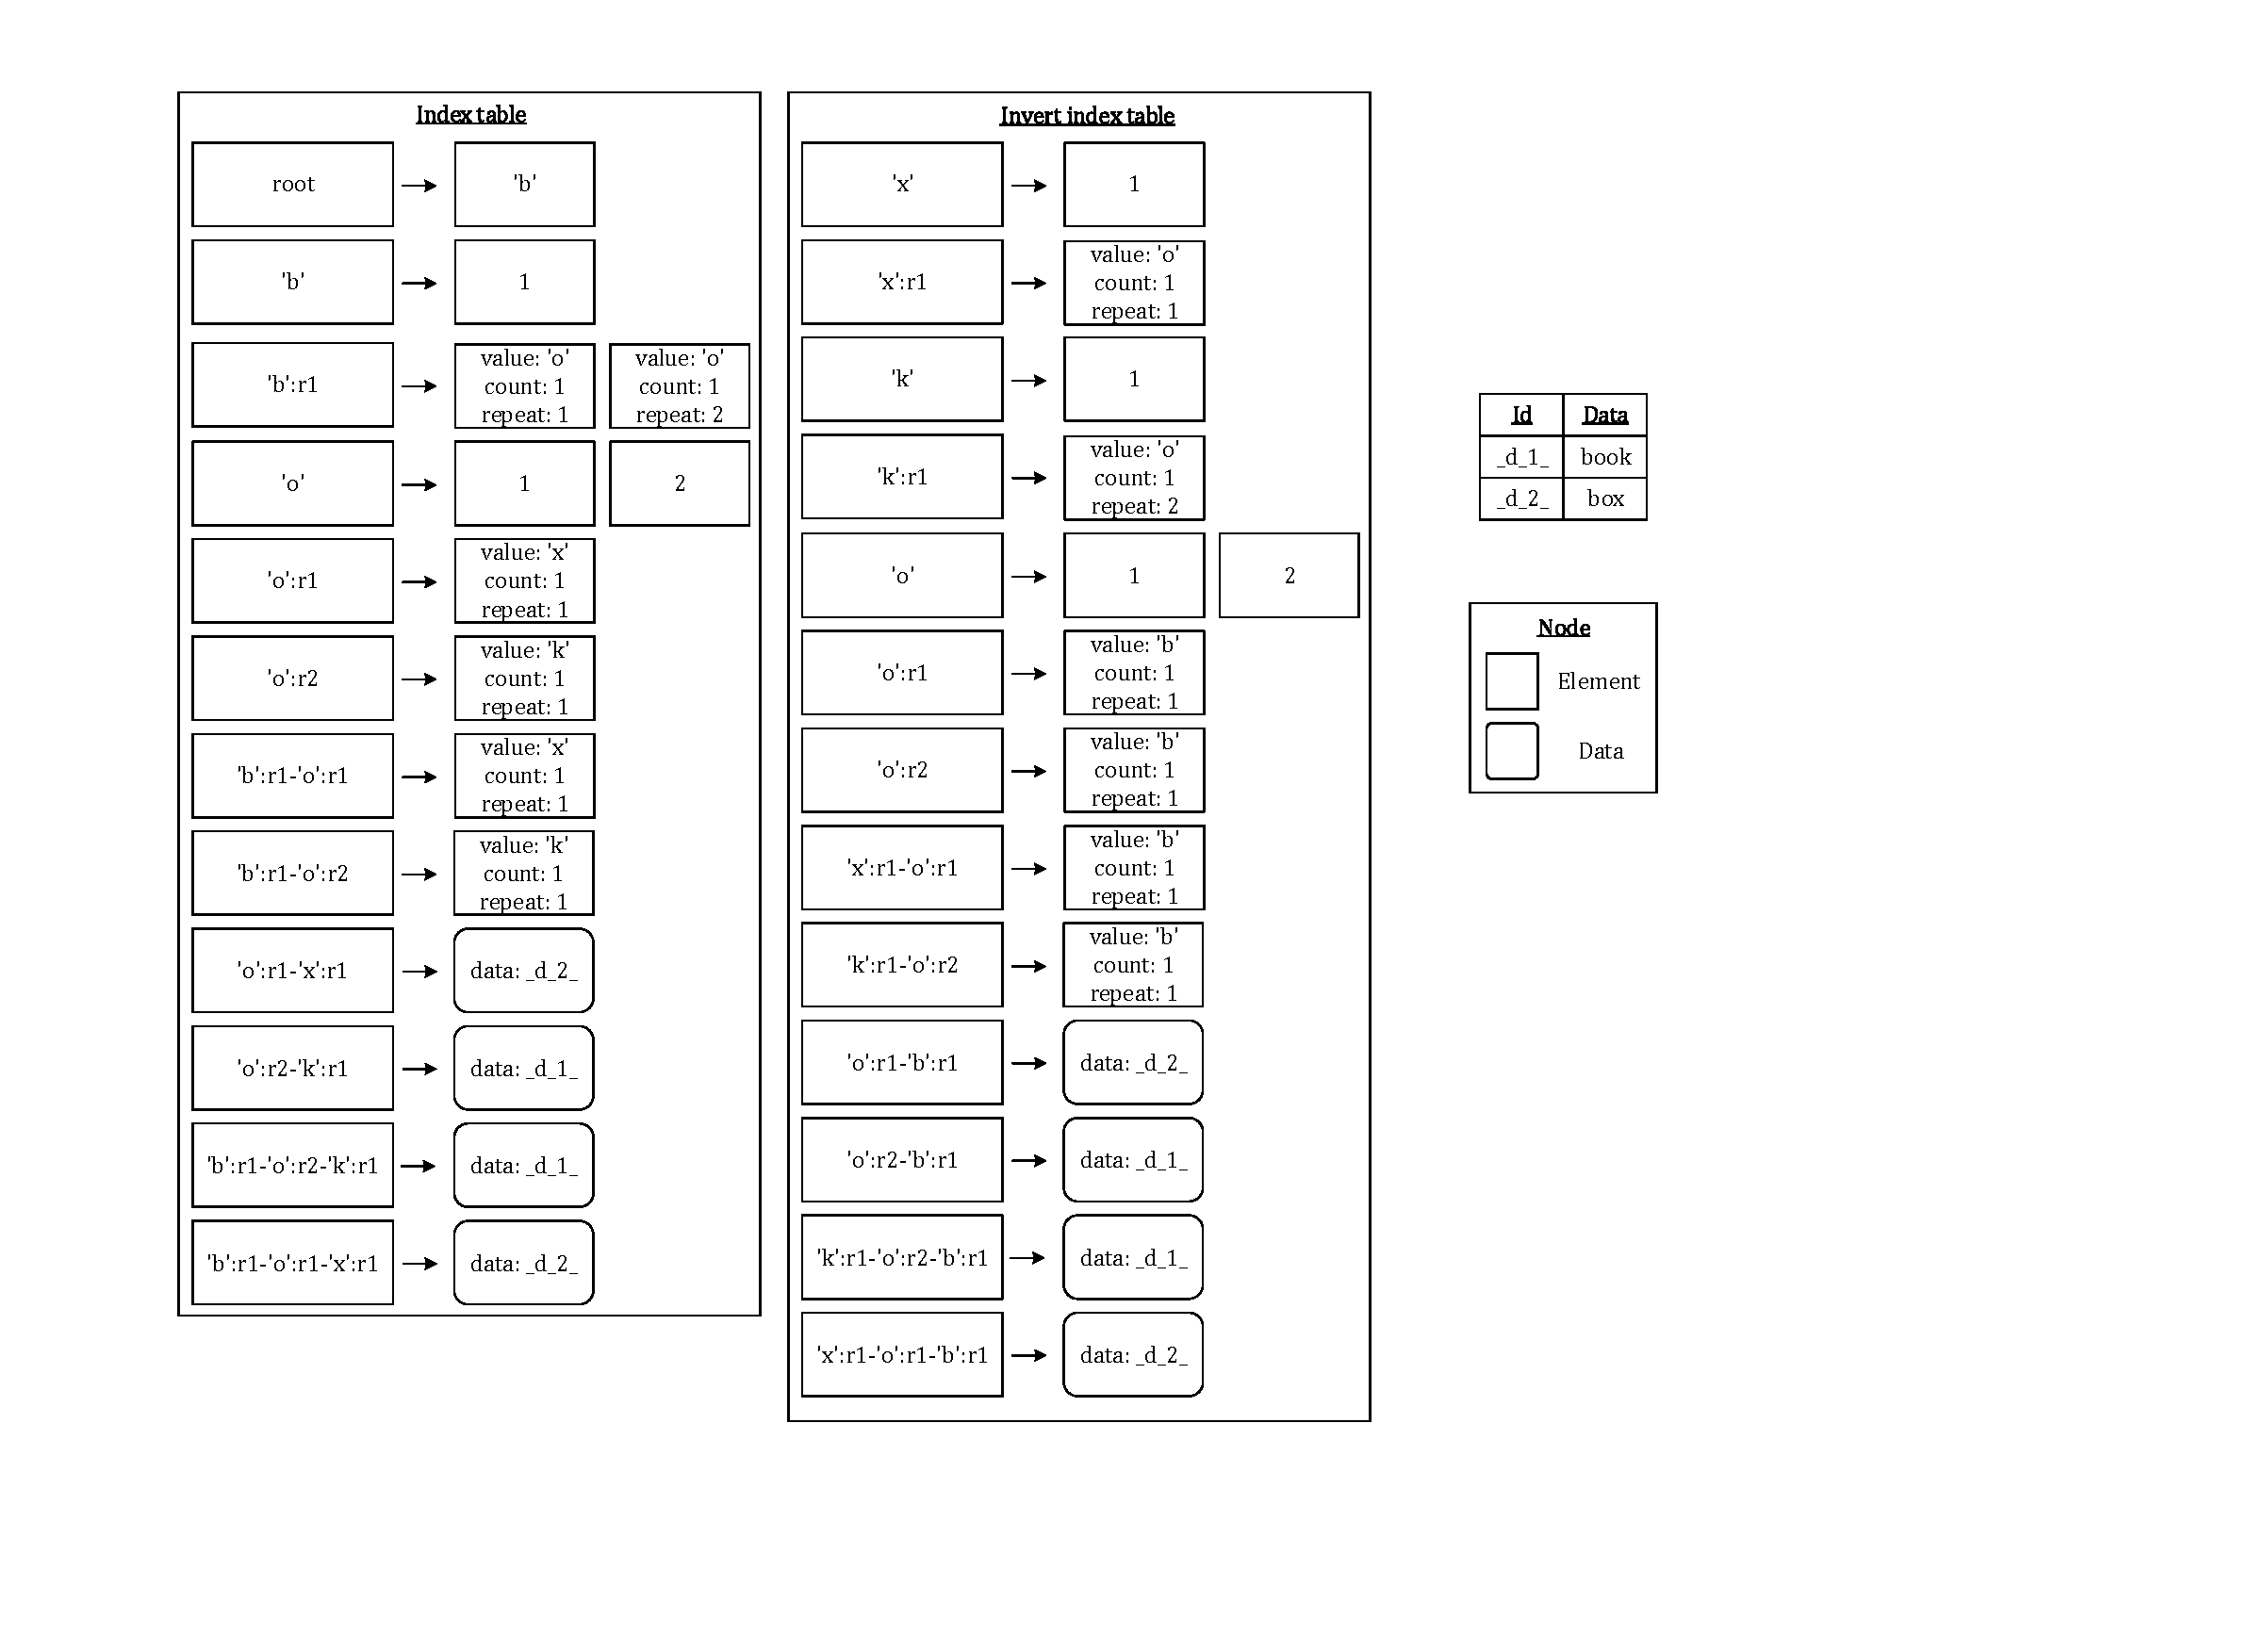
\includegraphics[width=0.8\textwidth]{./algorithm/string/pic/insertion/example_2_v5.pdf}
\caption{Insert data \textit{"box"}.}
\label{fig:algorithm:string:insertion:example_2}
\end{figure}

